% !TeX root = Stageportfolio.tex



\begin{landscape}
	\subsubsection{Les 17-18}
	\begin{tabularx}{1.56\textwidth}{|p{0.35\textwidth}|X|}\hline
		\textbf{Administratieve gegevens}\newline\newline
		Kevin Truyaert\newline\newline
		technisch secundair onderwijs\newline
		3e graad, 1ste jaar, Techniek-Wetenschappen\newline
		VVKSO: \href{http://ond.vvkso-ict.com/leerplannen/doc/Toegepaste\%20fysica-2014-041.pdf}{http://ond.vvkso-ict.com/leerplannen /doc/Toegepaste\%20fysica-2014-041.pdf} \newline
		\underline{Lesonderwerp}:\newline Oefeningen op de algemene inductiewet \& Toepassingen op inductie & \textbf{Doelstellingen}
		\begin{itemize}[itemsep=0.08\baselineskip]
			\item B27: Fluxverandering als oorzaak van inductiespanning toelichten
			\item B28: Met behulp van de wet van Lenz de zin van de inductiespanning vinden
			\item B29: De algemene inductiewet hanteren.
			\item B30: Het werkingsprincipe van een generator weergeven
		\end{itemize}
		\underline{Lesdoelen}\newline
		\vspace{-0.75cm}
		\begin{enumerate}[itemsep=0.08\baselineskip]
			\item De leerlingen kunnen de wet van Faraday-Lenz op een rechte, bewegende geleider toepassen.
			\item De leerlingen kennen de relatie tussen inductiespanning, magnetisch veld, lengte van de geleider, snelheid van de geleider en aantal windingen.
			\item De leerlingen kunnen de algemene inductiewet tijdens oefeningen hanteren.
			\item De leerlingen kunnen de werking van een wisselspanningsgenerator weergeven.
			
		\end{enumerate} \\\hline
	\end{tabularx}\vfill \textcolor{white}{.} 


	\begin{tabularx}{1.56\textwidth}{|p{0.55\textwidth}|X|}
		\hline
		\multirow{2}{0.55\textwidth}{\textbf{Beginsituatie}\newline  
		Er zijn acht leerlingen binnen 5TW. Er heerst een algemene klassfeer. De leerlingen hebben al theorie gekregen rond en basisoefeningen gemaakt op magnetische inductie.  \newline\newline NOG AANVULLEN MET LERAARKENMERKEN.} & \textbf{Acties}\newline\newline  
		- Ik wil oefeningen op zo'n wijze brengen dat ze steeds dezelfde structuur hebben. Die structuur bouw ik eerst samen met de leerlingen op, om ze daarna zelfstandig aan de slag te laten gaan met oefeningen die steeds wat complexer worden. \PinkHighlight{Tijdens het zelfstandig maken van de oefeningen probeer ik toch zeker}{13cm} \PinkHighlight{de zwakkere leerlingen in de gaten te houden en hen individueler te coachen bij het}{15cm} \PinkHighlight{maken van oefeningen.}{4.5cm}
		\newline\newline\newline\newline\newline\newline\newline\newline
		
		\\ \cline{2-2}
		  & \textbf{Bronnen}\begin{itemize}
		  	\item Schramme, S. (2018) De stroombalans, labo magnetisme 4
		  	\item Frederiksen (2014), Current Balance 4565.00
		  	\item Giancoli, D. C. (2008). Physics for scientists and engineers. Pearson Education International.
		  \end{itemize}\\ \hline
	\end{tabularx}


\newpage
	
	\begin{tabularx}{1.56\textwidth}{|p{1.5cm}|p{8cm}|X|p{4cm}|}
		\hline
		\textbf{Nr. lesdoel } & \textbf{Inhoud (timing)}  & \textbf{Organisatie } & \textbf{Media } \\ \hline
		1\newline\newline2\newline\newline3	&\underline{Oefeningen: de algemene} \underline{inductiewet (40 minuten)}\newline
			Tijdens deze lesfase focussen de leerlingen zich op het maken van oefeningen in verband met de algemene inductiewet. Deze combineert de wet van Faraday en de wet van Lenz, dus leerlingen moeten beide begrijpen om de oefeningen tot een goed einde te brengen. Tijdens deze oefeningensessie wil ik gebruik maken van correctiesleutels om de leerlingen hun oefeningen zelfstandig te laten corrigeren.
		&  \underline{Zelfstandig oefeningen maken} \underline{Bespreking via correctiesleutel}\newline 
			De leerlingen maken zelfstandig oefeningen 6 t.e.m. 11. Na het maken van iedere oefening kunnen ze een correctiesleutel ophalen waarin alle stappen beschreven staan. Zo kunnen de sterkere leerlingen zelfstandig meerdere (en complexere) oefeningen maken, terwijl ik mij concentreer op de zwakkere leerlingen. Wanneer ik zie dat er bij een bepaalde oefening klassikaal problemen zijn, kan ik bepaalde stappen op het bord brengen.
		&   Cursus hoofdstuk 5 p15-16\newline\newline Krijtbord
		\\ \hline
	\end{tabularx}\vspace{5mm}



\begin{tabularx}{1.56\textwidth}{|p{1.5cm}|p{8cm}|X|p{4cm}|}
	\hline
	\textbf{Nr. lesdoel } & \textbf{Inhoud (timing)}  & \textbf{Organisatie } & \textbf{Media } \\ \hline
    4 & \underline{Werking wisselspanningsgenerator:} \underlin{inleiding (5 minuten)}\newline
    	Opzet van de wisselspanningsgenerator verduidelijken en kennismaken met de werking ervan.
	&  \underline{Onderwijsleergesprek}\newline 
	Ik schets de opstelling van de wisselspanningsgenerator en vraag de leerlingen om alle componenten aan te duiden, te benoemen, \ldots 
	&  Cursus hoofdstuk 6 p6\newline\newline Slides
	\\ \hline
\end{tabularx}\vspace{5mm}


\begin{tabularx}{1.56\textwidth}{|p{1.5cm}|p{9cm}|X|p{4cm}|}
	\hline
	\textbf{Nr. lesdoel } & \textbf{Inhoud (timing)}  & \textbf{Organisatie } & \textbf{Media } \\ \hline
	4& \underline{Werking wisselspanningsgenerator:} \underline{eerste kwartdraai (5 minuten)}\newline
	De werking van de wisselspanningsgenerator wordt verduidelijkt. Dit zal in verschillende stappen gebeuren.
	&  \underline{Onderwijsleergesprek}\newline  De leerlingen kennen de werking van de algemene inductiewet. Via vraagstelling wil ik samen met hen de eerste kwartdraai van de wisselspanningsgenerator bespreken. Zo vullen we samen het eerste kader op pagina 7 in.
	&  Cursus hoofdstuk 6 p7\newline\newline Krijtbord
	\\ \hline
\end{tabularx}\vspace{5mm}


\begin{tabularx}{1.56\textwidth}{|p{1.5cm}|p{9cm}|X|p{4cm}|}
\hline
\textbf{Nr. lesdoel } & \textbf{Inhoud (timing)}  & \textbf{Organisatie } & \textbf{Media } \\ \hline
4& \underline{Werking wisselspanningsgenerator:} \underline{eerste kwartdraai (5 minuten)}\newline
De werking van de wisselspanningsgenerator wordt verduidelijkt. Dit zal in verschillende stappen gebeuren.
&  \underline{Onderwijsleergesprek}\newline  De leerlingen kennen de werking van de algemene inductiewet. Via vraagstelling wil ik samen met hen de eerste kwartdraai van de wisselspanningsgenerator bespreken. Zo vullen we samen het eerste kader op pagina 7 in.
&  Cursus hoofdstuk 6 p7\newline\newline Krijtbord
\\ \hline
\end{tabularx}\vspace{5mm}



\begin{tabularx}{1.56\textwidth}{|p{1.5cm}|p{9cm}|X|p{4cm}|}
	\hline
	\textbf{Nr. lesdoel } & \textbf{Inhoud (timing)}  & \textbf{Organisatie } & \textbf{Media } \\ \hline
	5\newline\newline 6& \underline{Magnetische fluxverandering:} \underline{Oefeningen (15 minuten)}\newline
	Aangezien de leerlingen net de eigenschappen van magnetische fluxverandering gezien hebben, maken we eerst wat oefeningen hierop. Die zijn essentieel om aan inductiespanning te kunnen beginnen.
	&  \underline{Onderwijsleergesprek + oefeningen}\newline  Oefening 7 maak ik klassikaal, met de leerlingen samen, via vraagstelling aan de leerlingen. Hierna werken de leerlingen individueel oefening 8 en 9. Ik schrijf enkel de tussenoplossingen en de eindoplossing op bord. Ondertussen plaats ik het materiaal voor de demo rond inductiespanning en -stroom op tafel.
	&  Cursus hoofdstuk 5 p5-6\newline\newline Krijtbord
	\\ \hline
\end{tabularx}\vspace{5mm}



\begin{tabularx}{1.56\textwidth}{|p{1.5cm}|p{9cm}|X|p{4cm}|}
	\hline
	\textbf{Nr. lesdoel } & \textbf{Inhoud (timing)}  & \textbf{Organisatie } & \textbf{Media } \\ \hline
	7\newline\newline 8& \underline{Inductiespanning en -stroom:} \underline{Inleiding (10 minuten)}\newline
	Er werd in vorige lessen (Hoofdstuk 2) door de leerlingen ondervonden dat een elektrische stroom een magnetisch veld veroorzaakt. Hier onderzoeken we of het omgekeerde ook waar is: induceert een magnetisch veld een elektrische stroom in een gesloten circuit? Dit zal een interactie tussen elektriciteit en magnetisme aan de leerlingen tonen.
	&  \underline{Demonstratie + Onderwijsleergesprek}\newline 
	De opstelling bestaat uit een spoel die aangesloten is aan een milliampèremeter, die zowel negatieve als positieve stromen kan meten. Daarna beweeg ik een magneet naar de spoel. Ik zeg niets en vraag aan de leerlingen wat zij beschrijven wat er gebeurt. Hier speel ik op in en treed ik in interactie met de leerlingen om van hen te horen wat zij ervaren wat er gebeurt.	Op basis hiervan interageer ik met de leerlingen om hen in hun bewoording te begeleiden. Hierna vullen we samen op basis van de demo pagina's 7 en 8 in.
	&  Cursus hoofdstuk 5 p7-8\newline\newline Krijtbord
	\\ \hline
\end{tabularx}\vspace{5mm}




\begin{tabularx}{1.56\textwidth}{|p{1.5cm}|p{9cm}|X|p{4cm}|}
	\hline
	\textbf{Nr. lesdoel } & \textbf{Inhoud (timing)}  & \textbf{Organisatie } & \textbf{Media } \\ \hline
	7\newline\newline 8\newline\newline 9& \underline{De wet van Faraday:} \underline{Verbanden (15 minuten)}\newline
	Er is nu aangetoond dat in een gesloten circuit er een inductie stroom is. We kunnen ditzelfde experiment doen, maar in plaats van een milliampèremeter aan de spoel aan te sluiten, sluit ik nu een voltagemeter aan. Hieruit is het mogelijk om de inductiespanning te meten door middel van een fluxverandering. Door verschillende wijzigingen aan de situatie toe te brengen, kunnen de leerlingen zelf bepaalde evenredigheden uit de demonstratie halen. Samen met de leerlingen leid ik de wet van Faraday af.
	&  \underline{Demonstratie + Onderwijsleergesprek}\newline 
	De opstelling bestaat uit een spoel die aangesloten is aan een voltagemeter, die zowel negatieve als positieve spanningen kan meten. Daarna beweeg ik een magneet naar de spoel. Ik zeg niets en vraag aan de leerlingen wat zij beschrijven wat er gebeurt. Hier speel ik op in en treed ik in interactie met de leerlingen om van hen te horen wat zij ervaren wat er gebeurt.	Deze resultaten zullen ze snel begrijpen, gezien we net de situatie van de inductiestroom gezien hebben. Nu verander ik de windingen van de spoel, de flux (door middel van de magneet) en de tijdspanne waarin ik de magneet dichter breng. Deze relaties leiden uiteindelijk tot de wet van Faraday. Hierna vullen we samen op basis van de demo pagina's 9 en 10 in.
	&  Cursus hoofdstuk 5 p9-10\newline\newline Krijtbord
	\\ \hline
\end{tabularx}\vspace{5mm}


\begin{tabularx}{1.56\textwidth}{|p{1.5cm}|p{9cm}|X|p{4cm}|}
	\hline
	\textbf{Nr. lesdoel } & \textbf{Inhoud (timing)}  & \textbf{Organisatie } & \textbf{Media } \\ \hline
	& \underline{Slot (5 minuten)}\newline
	Ik herhaal nog even kort samen met de leerlingen de wet van Faraday. We bespreken samen wat deze voorstelt, een inductiespanning, en waarop deze steunt, een fluxverandering. Op deze manier probeer ik de leerlingen te evalueren.
	&  \underline{Vertellen}\newline 
	Bespreken van de wet van Faraday en fluxverandering
	&  
	\\ \hline
\end{tabularx}




	
\end{landscape}


%\subsection*{Bijlage 5.1: slides introductie}

%
%\subsection*{Bijlage 1.2: bordschema theorie}
%\begin{center}
%	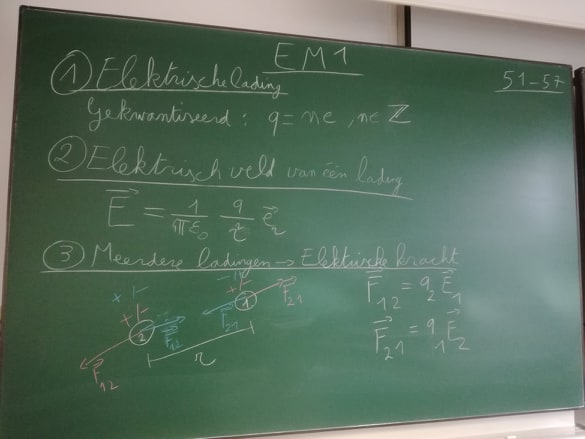
\includegraphics[width=0.9\textwidth]{Bord1a}
%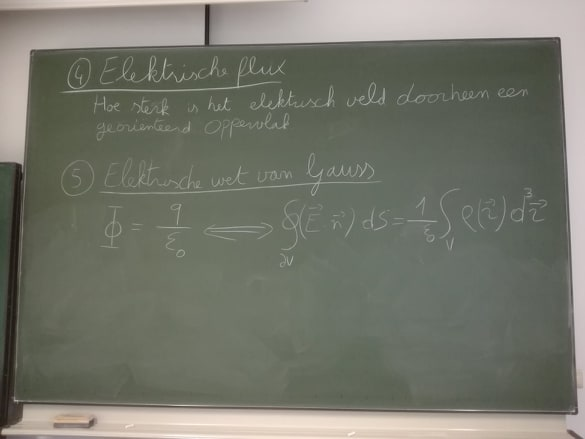
\includegraphics[width=0.9\textwidth]{Bord1b}
%\end{center}
%\newpage
%
%
%\includepdf[scale = 0.8,pages = 17,pagecommand=\subsection*{Bijlage 1.3: opgeloste oefeningen}]{Observaties_OpgelosteOef}
%\includepdf[scale = 0.8,pages =18-20,pagecommand=]{Observaties_OpgelosteOef}
%
%
%
%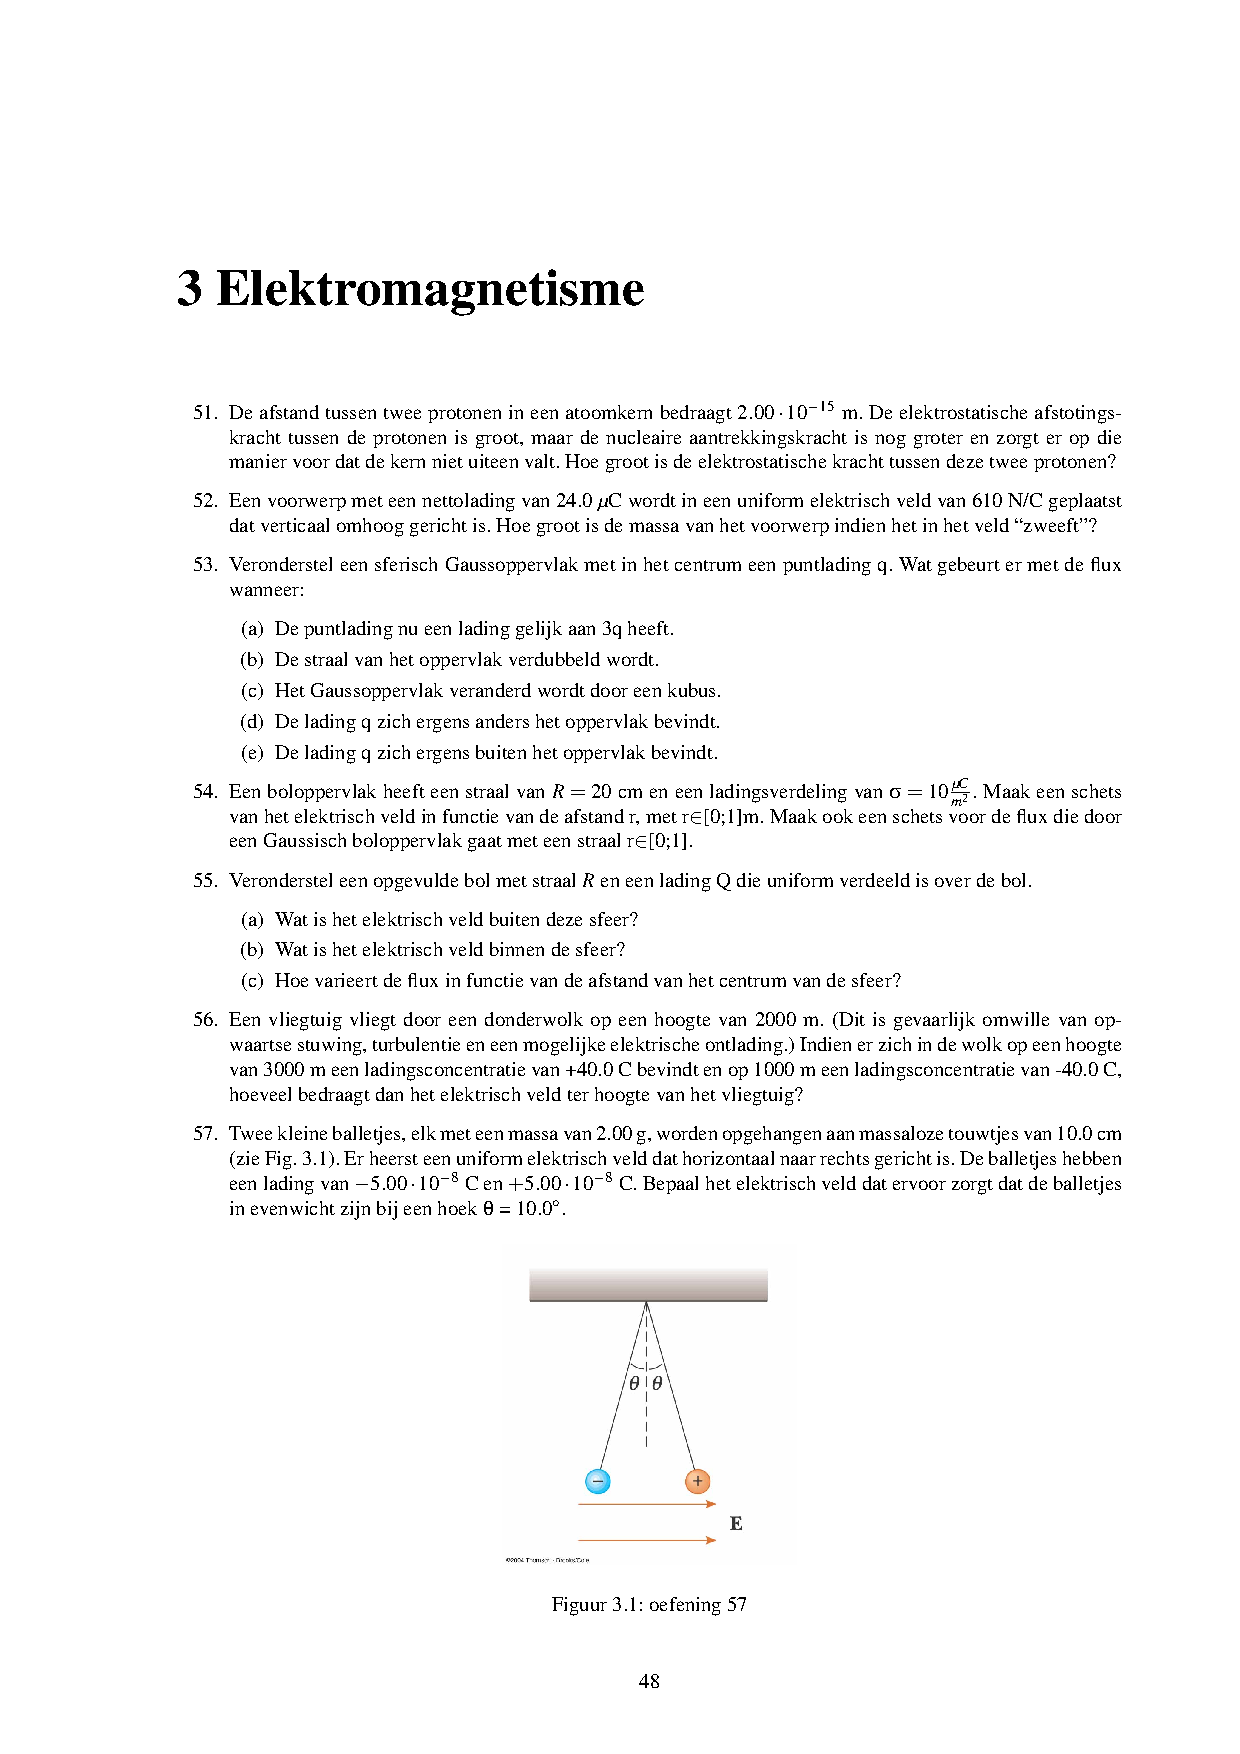
\includepdf[scale = 0.95,pages = 1,pagecommand=\subsection*{Bijlage 1.4: oefeningenbundel elektromagnetisme}]{OefeningenBundel}
%\includepdf[scale = 0.95,pages =2-,pagecommand=]{OefeningenBundel}